\section*{Problem \#22}


Given...

\begin{equation*}
    \begin{aligned}
        & \frac{C_{A}}{dt} = -r_{1} \\
        & \frac{C_{B}}{dt} = r_{1} - r_{2} \\
        & \frac{C_{C}}{dt} = r_{2}
    \end{aligned}
    \qquad \qquad
    \begin{aligned}
        & r_{1} = K_{1}C_{A} \\
        & r_{2} = K_{2}C_{B} \\
    \end{aligned}
\end{equation*}

We can define the states of system to be the concentrations of each species, in the reaction as follows...

\begin{equation*}
    \begin{aligned}
        & x_{1} = C_{A} \\
        & x_{2} = C_{B} \\
        & x_{3} = C_{C} \\
    \end{aligned}
\end{equation*}

From whose definitions we can construct a state space by taking first order time derivatives of each state, and substituting the appropriate expression from the equations given above. \\
$$
\begin{bmatrix}
    \dot{x_{1}} \\
    \dot{x_{2}} \\
    \dot{x_{3}}
\end{bmatrix}
=
\begin{bmatrix}
    -K_{1} & 0 & 0 \\
    K_{1} & -K_{2} & 0 \\
    0 & K_{2} & 0
\end{bmatrix}
\begin{bmatrix}
    x_{1} \\
    x_{2} \\
    x_{3} \\
\end{bmatrix}
$$

Such that a matrix $A$ is define to be...

$$
A =
\begin{bmatrix}
    -K_{1} & 0 & 0 \\
    K_{1} & -K_{2} & 0 \\
    0 & K_{2} & 0
\end{bmatrix}
$$

\subsection*{22.A}
Since we can the constitutive equations for the system are a linear function of its arguments, this problem is \textbf{linear system}, and consequently can be written in matrix form as shown above.

\subsection*{22.B}

Since the system is linear, it can be written via the matrix equation shown below...


    $$    \dot{x} = Ax + Bu \\$$
    $$    y = Cx + Du \\$$

\noindent Where the matrices $A$ and $B$, descripe the state and input dynamics of the system, while matrices $C$ and $D$ describe the outputs of the system.

\begin{equation*}
    \begin{aligned}
        & A =
        \begin{bmatrix}
            -K_{1} & 0 & 0 \\
            K_{1} & -K_{2} & 0 \\
            0 & K_{2} & 0 \\
        \end{bmatrix}
        & B =
        \begin{bmatrix}
            0 \\
            0 \\
            0
        \end{bmatrix}
    \end{aligned}
    \qquad \qquad
    \begin{aligned}
        & C =
        \begin{bmatrix}
            1 & 0 & 0
        \end{bmatrix}
        & D =
        \begin{bmatrix}
            0 \\
        \end{bmatrix}
    \end{aligned}
\end{equation*}


\subsection*{22.C}

The dynamics of the response due to its ``initial conditions'' is shown below for all three states of the system, even though the output of the system can only measure the $X_1$. \\


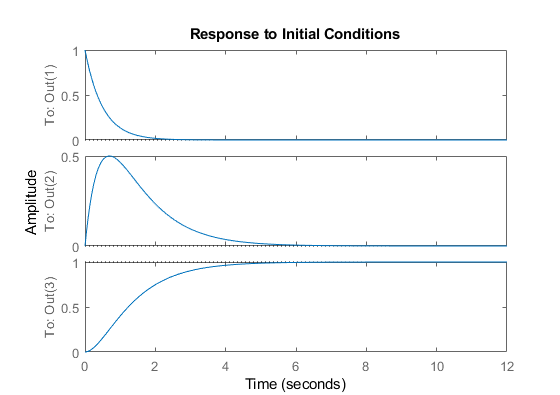
\includegraphics{ss_sim}
